\documentclass[12pt]{book}
\usepackage[width=4.375in, height=7.0in, top=1.0in, papersize={5.5in,8.5in}]{geometry}
%\usepackage[pdftex]{graphicx}
\usepackage{amsmath}
\usepackage{amssymb}
\usepackage{tipa}
%for using the euro sign
\usepackage{eurosym}
\usepackage{graphicx}
%\usepackage{txfonts}
\usepackage{textcomp}
%\usepackage{amsthm}
%\usepackage{array}
%\usepackage{xy}
\usepackage{fancyhdr}

\usepackage{hyperref}

%The below is used for codes
\usepackage{listings}
\usepackage{color}

\definecolor{dkgreen}{rgb}{0,0.6,0}
\definecolor{gray}{rgb}{0.75,0.75,0.75}
\definecolor{mauve}{rgb}{0.58,0,0.82}

\lstset{
  backgroundcolor=\color{gray},  % choose the background color; you must add \usepackage{color} or \usepackage{xcolor}
  basicstyle=\footnotesize,       % the size of the fonts that are used for the code
  breakatwhitespace=false,        % sets if automatic breaks should only happen at whitespace
  breaklines=true,                % sets automatic line breaking
  captionpos=b,                   % sets the caption-position to bottom
  commentstyle=\color{dkgreen},   % comment style
  deletekeywords={...},           % if you want to delete keywords from the given language
  escapeinside={@}{@)},         % if you want to add LaTeX within your code
  extendedchar=true,              % lets you use non-ASCII characters; for 8-bits encodings only, does not work with UTF-8
  frame=single,                   % adds a frame around the code
  keywordstyle=\color{mauve},      % keyword style
  language=C,                % the language of the code
  morekeywords={*,...},           % if you want to add more keywords to the set
  numbers=left,                   % where to put the line-numbers; possible values are (none, left, right)
  numbersep=5pt,                  % how far the line-numbers are from the code
  numberstyle=\tiny\color{dkgreen},  % the style that is used for the line-numbers
  rulecolor=\color{gray},        % if not set, the frame-color may be changed on line-breaks within not-black text (e.g. comments (green here))
  showspaces=false,               % show spaces everywhere adding particular underscores; it overrides 'showstringspaces'
  showstringspaces=false,         % underline spaces within strings only
  showtabs=false,                 % show tabs within strings adding particular underscores
  stepnumber=1,                   % the step between two line-numbers. If it's 1, each line will be numbered
  stringstyle=\color{mauve},      % string literal style
  tabsize=4,                      % sets default tabsize to 2 spaces
  title=\lstname                  % show the filename of files included with \lstinputlisting; also try caption instead of title
}
%until here

\newcommand{\tab}{\hspace*{2em}}


\pagestyle{fancy}
\renewcommand{\chaptermark}[1]{\markboth{#1}{}}
\renewcommand{\sectionmark}[1]{\markright{\thesection\ #1}}
\fancyhf{}
\fancyhead[LE,RO]{\bfseries\thepage}
\fancyhead[LO]{\bfseries\rightmark}
\fancyhead[RE]{\bfseries\leftmark}
\renewcommand{\headrulewidth}{0.5pt}
\renewcommand{\footrulewidth}{0pt}
\addtolength{\headheight}{0.5pt}
\setlength{\footskip}{0in}
\renewcommand{\footruleskip}{0pt}
\fancypagestyle{plain}{%
\fancyhead{}
\renewcommand{\headrulewidth}{0pt}
}
%
%\parindent 0in
\parskip 0.05in
%
\begin{document}
\frontmatter
\pagestyle{empty}
%\pagenumbering{}
% Set book title
\title{\textbf{A course on Wireless Sensor Networks (WSNs)}}
% Include Author name and Copyright holder name
\author{Luis Sanabria, Jaume Barcelo}
% 1st page for the Title
%-------------------------------------------------------------------------------
\maketitle
%
\tableofcontents
%
\mainmatter
%
\chapter{About the course}

\section{Course Data}

Code: 21754

Course name: ``Xarxes de Sensors Sense Fils''

Teacher: Luis Sanabria and Jaume Barcelo

Credits: 4

Year: 3rd or 4th year (optional)

Trimester: Spring

\section{Introduction}
The reduction in price and size of computing and wireless communication platforms over the last years opens a new possibility for gathering and processing information: Wireless Sensor Networks.
A wireless sensor node is an electronic device of small dimensions that gathers measures from the environment and transmit the data wirelessly.
In wireless sensor nodes, communication is often established with other wireless sensor nodes to exchange or pass information.
It is common to have this data directed to an special device that gathers all the data and is called the network sink.
As wireless sensor nodes are often battery-powered, energy saving is a relevant issue in these networks.

What follows is an extract of the first pages of \cite{sanabria2012lpw}.

\begin{quotation}
Wireless Sensor Networks (WSNs) are a result of significant breakthroughs on wireless transceiver technology, the need of event sensing and monitoring. One might think of a WSN as the skin of our bodies; apart from its importance on many other subjects, our skin senses events nearby it, like touch, temperature changes, pressure and so forth. These events are generated by an external entity, the nerves or sensors of our skin are capable to react to such events and transmit this information to the brain. \\

There are enormous differences among characteristics of WSN and the skin, but the example given above will work as head start to understanding the technology. For instance, our skin sends the sensed event information towards the brain through the nerves, we could safely relate this medium to a wired network infrastructure. While in WSN, as its name suggests sends the sensed data towards a central node (Sink) via a wireless medium. Because of the limited radio range of each node, the route to the Sink is generally composed of jumps through different nodes (which is called a multi-hop route).\\

The majority of wireless nodes in a WSN are very constrained devices due to the restrictions in costs and sometimes harsh environments where these networks are deployed. These constraints go from cost, processing power, memory, storage, radio range, spectrum and, more importantly, battery life. One of the most popular low-end nodes model, the TelosB, is equipped with $16$ MHz CPU, very small flash memory ($48$ KB avg.), about $10$ KB of RAM and works on the very crowded $2.4$ GHz spectrum at rates around $250$ Kbps. These limitations force WSN engineers to design applications capable of working with low processor-intensive tasks and powered with limited battery (usually two AA batteries).\\

Many WSN applications process the sensed event before sending the data, this processing tries to reduce the information to send. As mentioned in \cite{akyildiz2010wireless}, it is less energy consuming to process one bit of information than sending it. WSN protocols and applications are tailored to power conservation rather than throughput, mainly due to cost, dimension, processing and power constraints.\\

WSNs may contain different kind of sensors that help monitor metrics related to: temperature, humidity, pressure, speed, direction, movement, light, soil makeup, noise levels, presence or absence of certain kinds of objects, mechanical stress and vibration. Also further information like node location can be derived from a Global Positioning System (GPS) device embedded at each node.\\

Because of the variety of measures than can be monitored with these small and (generally) cheap devices, a wide range of applications have been developed; the authors of \cite{akyildiz2010wireless} divide them in: military, environmental, health, home and industry applications.\\

\begin{itemize}
    \item \emph{Military Applications:} one of the first applications of WSNs. The main advantages in this area are the fact that the deployment of low cost sensors (that are subject to destruction in a battlefield) proposes a cheaper approach to sensing different types of metrics, which in turn brings new challenges to WSN applications (increased power and processing constraints). Some of the applications are related to: monitoring the movement of troops, equipment and ammunition, battlefield surveillance, terrain reconnaissance, damage assessments, snipper detection \cite{ledeczi2005countersniper}, \cite{mazurek2005boomerang} and threat detection, as in the case of biological, radiological or chemical attacks.\\
    \item \emph{Environmental Applications:} most of these applications are related to animal tracking, weather conditions and threat contention \cite{polastre2004analysis}, \cite{szewczyk2004habitat}.\\
    \item \emph{Health Applications:} a great deal of these applications are dedicated to monitor patients inside hospitals and provide them with better care. This is achieved by tracking the patientÕs vitals or other information of interest and making it available to doctors at any time from anywhere securely through the Internet. \\
    \item \emph{Home Applications:} technology is making its way inside our homes from various fronts, and WSN are no exception. Sensor nodes inside domestic devices will result in an increased interaction among them and allow access via the Internet. Theses applications are of great importance in fields like domotics towards a smart home/work environment. Home surveillance and multimedia WSNs for home environments are also a growing field of research.\\
    \item \emph{Industrial Applications:} historically the monitoring of material fatigue was made by experts introducing the observed situation inside PDA devices to be collected on a central site for processing. Further sensing techniques were developed on the form of wired sensors; nevertheless its implementation was slow and expensive due the necessary wiring. WSNs bring the best of both methods by sensing the events without the need of expert personnel and the cost of wiring. \\
    \item Other implementations as mentioned in \cite{akyildiz2010wireless} are: inventory management, product quality monitoring, smart offices/houses; guidance in automatic manufacturing environments, interactive museums, factory process control and automation, machine diagnosis, transportation, vehicle tracking and detection, spectrum sensing for cognitive radio networks, underground and underwater monitoring. \\
\end{itemize}

\end{quotation}

\section{Syllabus}
\begin{itemize}
  \item Lectures
  \begin{enumerate}
    \item Introduction to WSNs.
    \item Arduino Platform.
    \item XBee and XBee explorer. AT commands.
    \item XBee API mode.
    \item A sensor network with Arduino.
    \item A sensor network without Arduino.
    \item Publishing sensed data
    \item Invited talk
    \item Quiz
  \end{enumerate}
  \item Labs and seminars
  \begin{enumerate}
    \item Blinking LED (Dimming optional)
    \item Blinking LED with push-button (dimming optional)
    \item XBee chat
    \item Wireless doorbell
    \item Sunset sensor
    \item Sensor network with Arduino
    \item Sensor network with XBee in API mode
    \item Sleeping and actuating
    \item Uploading sensed data to the Internet
  \end{enumerate}
\end{itemize}

\section{Bibliography}

Most of the lab assignments follow the book that you can find at the university library:

Robert Faludi ``Building Wireless Sensor Networks'' (\cite{faludi2010bws}).

The following list of ``common mistakes'' can be very useful when debugging your projects:

\url{http://www.faludi.com/projects/common-xbee-mistakes/}

Check also:

Massimo Banzi ``Getting Started with Arduino''.

\section{Evaluation Criteria}

The grading is distributed as follows:
\begin{itemize}
\item Quiz, 10\%
\item Each lab assignment, 10\%
\end{itemize}

It is necessary to obtain a decent mark in all the different evaluation aspects.
To pass the course, 50 out of the total 100 points need to be obtained.

\section{Team work}

You will work in teams of three people.
Try to make the groups as heterogeneous as possible: people that are experienced with Arduino and people that are not, people from different majors, people with strong programming skills and people good at electronics, etc.

Each group delivers a single report per session and the teachers may ask questions to individual members of the team.

\section{Use your imagination}
The lab assignments are somewhat easy.
The goal is that you complement what you do in the lab with other ideas of your own.
You are encouraged to explore WSNs beyond the basics introduced in the assignments and document your findings in the reports.
Doing something on your own beyond the assignment takes a lot of effort and is time-consuming.
Nevertheless, as engineers, we should be able to come up with new ideas and solutions on our own.

\section{Non-stop Arduino}
In our school there are two additional courses that make use Arduino: ``Sensors and data acquisition'' and ``Interactive Systems''.

\section{Survival guide}

\subsection{Questions and doubts}
We like to receive questions and comments.
Normally, the best moment to express a doubt is during the class, as it is likely that many people in the class share the same doubt.
If you feel that you have a question that needs to be discussed privately, we can discuss it right after the class.

\subsection{Continuous feedback}
At the end of the lecture, we will ask you to anonymously provide some feedback on the course \emph{\color{blue}{\href{http://bit.ly/10tXjX4}{using a form like this one}}}.
In particular, I always want to know:
\begin{itemize}
\item What is the most interesting thing we have seen in class.
\item What is the most confusing thing in the class.
\item Any other comment you may want to add.

In labs, I will ask each group to hand in a short (few paragraphs) description of the work carried out in class, and the members of the group that have attended the class.
Note that this is different from the deliverables, which are the ones that are actually graded.
\end{itemize}

\subsection{How to make you teachers happy}

Avoid speaking while we are talking.

\chapter{Introduction to Arduino}

\section{Open Hardware}
\emph{"There's a fine line between open source and stupidity"}, says Massimo Banzi to a reporter from Wired Magazine while having dinner at a restaurant in Milan. 

Banzi is the man behind Arduino, an open hardware platform. The open about it relates to the fact that the device's manufacturing schematics, programming language and software development environment are free and open source. This basically means that everyone interested on building hardware-coupled solutions may take an Arduino board's schematics, modify it at will, send the new design to a China manufacturer and get the final product back home for around \EUR{10}~\cite{wiredOpenHardware}.

Open hardware is supported by a variety of available licenses (like open software with LGPL, GPL, Copyleft, and others) that ensure that the protected platform can be copied, enhanced and even sold, but always recognizing the original authors. It also ensures that the resulting products are open as the original.

\section{The Arduino Platform}
Arduino was developed to teach Interaction Design~\cite{banzi2008getting}, that meant that it required the ability to sense the surroundings and do something about it.

The platform is equipped with simple digital and analog input/output interfaces, that can be programmed to sense or react to some events. Figure~\ref{fig:ArduinoBoard} shows the Arduino Duemilanove board.

\begin{figure}[htbp]
  \centering
  \includegraphics[width=0.7\linewidth]{figures/duemilanove.eps}
  \caption{Arduino Duemilanove board
  \label{fig:ArduinoBoard}}
\end{figure}

There are numerous sensors and actuators that work with Arduino. In relation to sensors: temperature, air pollution, light, GPS modules and sound are among the popular; as LEDs, speakers and digital/analog outputs are common actuators. Also, interfaces like buttons can be programmed and used as a human interactive input.

The design and electrical components of the Arduino board are available for anyone~\cite{Arduino}. Figure~\ref{fig:Arduino_schematics} shows the connections layout of the Duemilanove model (see Figure~\ref{fig:ArduinoBoard}).

\begin{figure}[htbp]
  \centering
  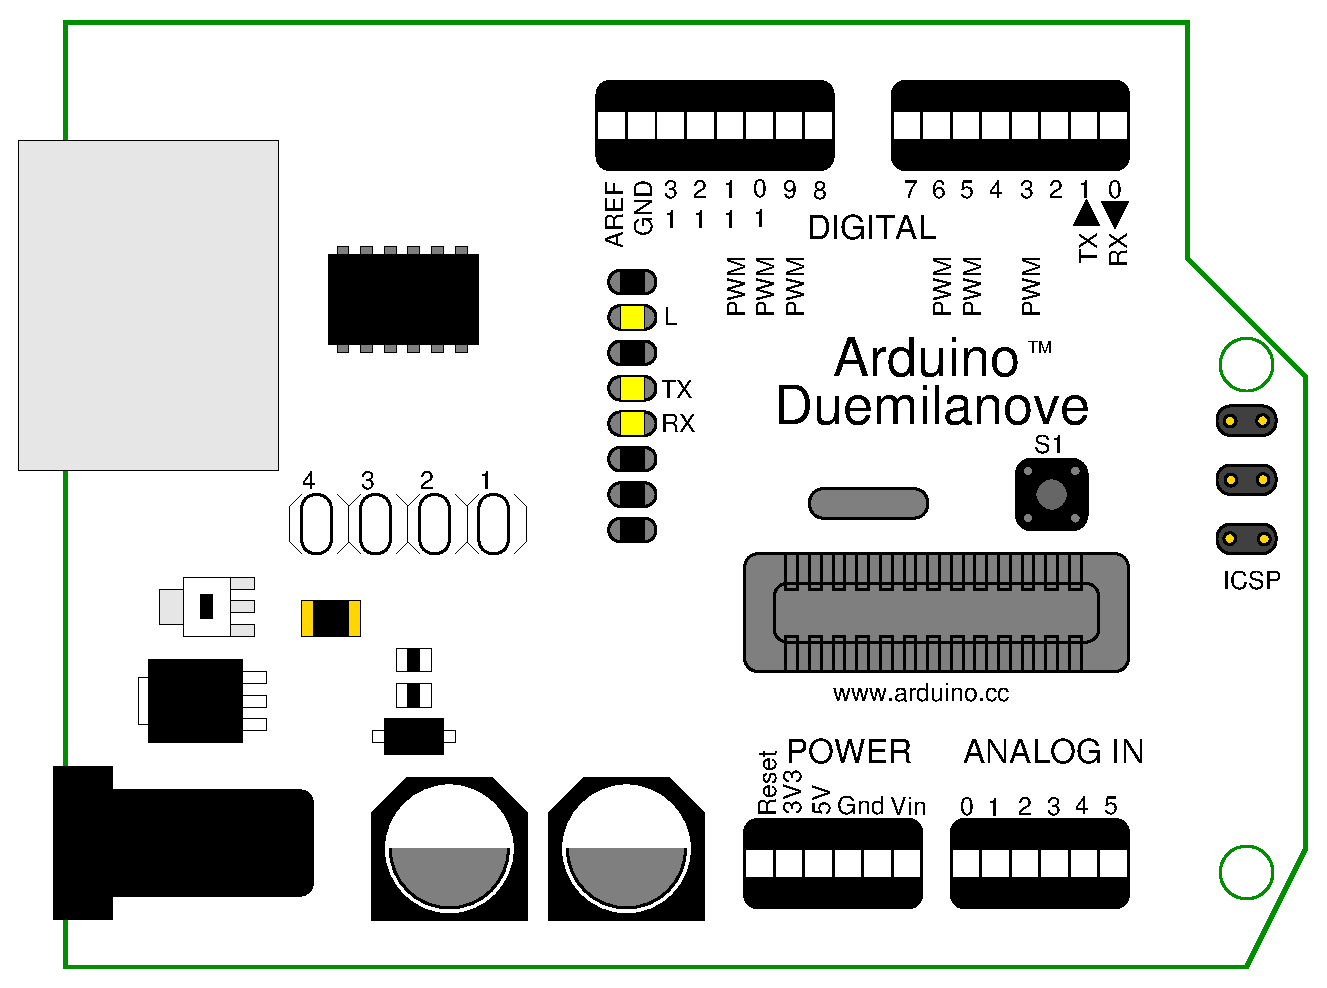
\includegraphics[width=0.7\linewidth]{figures/duemilanove_layout.eps}
  \caption{Arduino Duemilanove board: layout
  \label{fig:Arduino_schematics}}
\end{figure}

% \subsection{Developing for Arduino}

% \subsection{Example of a simple Arduino application}
	\chapter{Practice: Installing the Arduino IDE}\label{pract:settingTheIDE}
\section*{Suggested read: Chaper~ \ref{introToArduino}}

In the following practice, you will spend some time getting to know the Arduino platform, its connections and how to interact with it through a PC.

\section{Reviewing the hardware}\label{pract:settingTheIDE:hardware}
As you were able to see in Figure~\ref{fig:Arduino_schematics}, the Arduino board contains a whole computer on a small chip, although it is at least a thousand times less powerful.

Taking a closer look at Figure~\ref{fig:Arduino_schematics}, you will be able to see \emph{14 Digital IO pins (pins 0-13), 6 Analogue IN pins (0-5) and 6 Analogue OUT pins (pins 3, 5, 6, 9, 10, and 11)}.

The \emph{Digital IO} pins, as the name suggests can be set to input or output. Their function is specified by the sketch you create in the IDE (more on IDE in Section~\ref{pract:settingTheIDE:IDE}). The \emph{Analogue IN} ports take analogue values (i.e., voltage readings from a sensor) and convert them into a number between 0 and 1023. As for the \emph{Analogue OUT} ports, are actually digital pins that can be reprogrammed for analogue output using the sketch you can create in the IDE.

\section{The Arduino IDE}\label{pract:settingTheIDE:IDE}
The Arduino Integrated Development Environment (IDE) is the responsible for making your code work in the Arduino board. Without entering in much unnecessary detail, what the IDE does is to translate your code into C language and compile it using \texttt{avr-gcc}, which makes it understandable to the micro-controller. This last step hides away as much as possible the complexities of programming micro-controllers, so you can spend more time thinking on your actual code.

You can download the Arduino IDE~\emph{\color{blue}{\href{http://www.arduino.cc/en/Main/Software}{from here}}}. If you are using \emph{Linux} or \emph{Windows} operating systems, just double click the downloaded file. This will open a folder named \emph{arduino-[version]}, such as \emph{arduino-1.0}. Place the folder wherever you want in your system. For Ubuntu users, a good alternative is to use the \emph{Ubuntu Software Center} when available. On the Mac, just double click the downloaded file, this will open a disk image containing the Arduino application. Drag a drop the application icon to your Applications folder.

Do not open your installed application yet. First you must teach your computer to detect the Arduino hardware through the USB ports.

\subsection{Configuring the USB ports for detecting the Arduino}
In Linux and OS X, the USB controllers are the same used by the operating system.

\emph{\bf{On the Mac}}, plug the Arduino into an USB port.

The PWR light on the board should come on. Also, the LED labelled "L" should start blinking.

Then, a pop-up window telling you that a new network interface was found should appear. Proceed clicking "Network Preferences...", and then "Apply". Although it may appear with a status of "Not Configured", the Arduino is ready for work.

\emph{\bf{Windows}} machines, plug your Arduino and the ``Found new Hardware Wizard'' will appear. After the wizard tries to find the driver on the Internet, you will be able to select "Install from a list or specific location" button. Choose it and click next. You will be able to find the drivers under the "Drivers" folder of the Arduino Software download.

Once the drivers are installed, you can launch the IDE and start using Arduino.

\subsection{Identifying the port connected to the Arduino}
In the case of the \emph{\bf{Mac}}, once in the Arduino IDE, select "Serial Port" from the "Tools" menu. Select \texttt{/dev/cu/.usbmodem}; this is the name that your computer uses to refer to the Arduino board.

For \emph{\bf{Windows}}, under the operating system "Start" menu open the "Device Manager" by right-clicking on "Computer" (Vista) or "My Computer" (XP), then choose properties. On XP, click "Hardware" and choose Device Manager. On Vista, click "Device Manager".

Look for the Arduino device in the list under "Ports (COM \& LPT)". Your device name will be followed by a port number, usually "COM\#", where \# refers to a number.

Once you have identified the COM port number for the Arduino connection, you can select that port from the Tools~$>$~Serial Port menu in the Arduino IDE.

Now the Arduino IDE can talk with the Arduino board and program it.

\subsection{What's the deal with Linux users?}
As mentioned before, IDE uses the same USB controllers than Linux. So, in order to effectively detect your Arduino in Linux, simply connect it to your PC, open a Terminal a type \texttt{ls /dev/tty*}. This will display all available ports. Your Arduino serial port will probably be something like \texttt{/dev/ttyUSB0} or \texttt{/dev/ttyACM0}, but you can be sure by typing \texttt{dmesg} in the Terminal and looking at the line that details the last connected USB device to a determined \texttt{/dev/tty*} port.
	\chapter{Practice: Blinking LED}\label{pract:blinkingLED}
\section*{Suggested read: Chapers~\ref{introToArduino}~and~\ref{pract:settingTheIDE}}

In the following practice you will write your first Arduino application. Although simple, mastering it will provide you with clear understanding of the IDE and the components that conform the Arduino platform.

It consist of a simple code that will turn on/off LED(s) plugged to the digital IO ports of the Arduino.

\section{Preparing your development environment}
For Practice~\ref{pract:blinkingLED}, you will need:
\begin{itemize}
 \item as many LEDs as you want, but always less than the number of digital IO ports.
 \item a USB cable to connect your Arduino board to the PC.
 \item the Arduino IDE, up and running.
\end{itemize}

Turn your Arduino on by plugging it to the PC. Make sure you have selected the appropriate COM port, as it is explained in Practice~\ref{pract:settingTheIDE} according with your operating system.

\section{The code} 
Once inside, enter the following code:

\begin{lstlisting} [caption = {Blinking LED example code}, language = C, label = {code:blinkingLED}, numbers = left, escapeinside={@}{@}]
const int LED = 13; @\label{BL:LED}@

void setup() @\label{BL:SETUP}@
{
	pinMode(LED,OUTPUT); @\label{BL:pinMODE}@
}

void loop() @\label{BL:LOOP}@
{
	digitalWrite(LED, HIGH); @\label{BL:HIGH}@
	delay(1000); @\label{BL:DELAY}@
	digitalWrite(LED, LOW); @\label{BL:LOW}@
	delay(1000); @\label{BL:DELAY2}@
}
\end{lstlisting}

As you might be able to see, the code is completely readable. Let's review it line by line.

\begin{itemize}
	\item Line~\ref{BL:LED}: \texttt{const int LED = 13}, assigns the value $13$ to a \texttt{\color{red}{int}}erger variable, named LED. In this case, this number corresponds to the digital IO port \#13.
	\item Line~\ref{BL:SETUP}: \texttt{void setup()} is the name of the next block of code. It is very similar to functions in languages like C/C++ and it is generally used to assign variables to ports, as well as their role.
	\item Line~\ref{BL:pinMODE}: \texttt{pinMode(LED,OUTPUT)} tells the Arduino how to set the pins. In this case, pin LED ($\#13$) is set up as an OUTPUT. \texttt{pinMode} is a function, and the words or numbers inside the parenthesis are its arguments.
	\item Line~\ref{BL:LOOP}: \texttt{void loop()}: is where you define the behaviour of your device. The statements contained in \texttt{loop()} are repeated over and over again until the device is turned off.
	\item Line~\ref{BL:HIGH}: \texttt{digitalWrite(LED, HIGH)} works as a power socket for pins. In this case, the command is indicating to turn pin \texttt{LED} into \texttt{HIGH}, which instructs Arduino to turn the output pin to $5$V. If you have connected a LED in this pin, the result is that it will turn on (hopefully). Turning on and off the pin allow us to see what the software is making the hardware do; the LED is an actuator.
	\item Line~\ref{BL:DELAY}: \texttt{delay(1000)} tells the processor to wait for $1000$ \emph{milliseconds} before proceeding to the next code line.
	\item Line~\ref{BL:LOW}: \texttt{digitalWrite(LED, LOW)} as with Line~\ref{BL:HIGH}, this function turns pin \texttt{LED} to $0$V, causing the connected LED to turn off. You can do a mental map in which $HIGH \rightarrow ON,\ LOW \rightarrow OFF$.
	\item Line~\ref{BL:DELAY2}: because the last instruction was to set the LED off, this will keep it that way for an additional $1000$ \emph{millisecods}.
\end{itemize}

To see your work, just insert the longer leg of the LED into the digital IO port you assigned to variable \texttt{LED} on your code (digital pin $13$), and the shorter leg to ground (GND). Figure~\ref{fig:blinkingLEDLayout} shows the desired layout.

\begin{figure}[htbp]
  \centering
  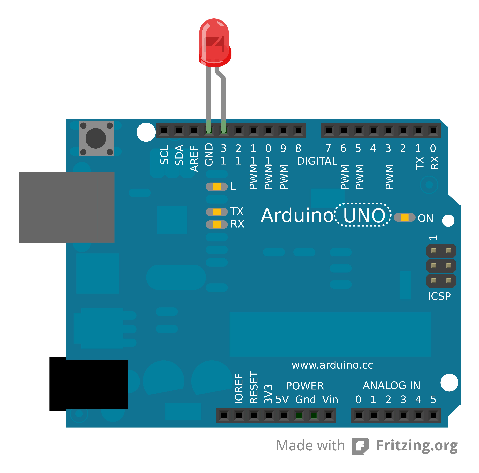
\includegraphics[width=0.7\linewidth]{figures/blinkingLED-NEW.eps}
  \caption{Blinking LED layout
  \label{fig:blinkingLEDLayout}}
\end{figure}

	\section{Practice: Blinking LED Advanced}\label{pract:blinkingLEDAdvanced}

It will be very boring to just have a blinking LED. That is because in this practice we will be incorporating some hardware and software tweaks that will allow us to have a little more control over the LED. Or let's say, we will make a basic lamp.

What we want to prototype is a LED that turns on or off whenever we press a bottom. Before we dwell into detail, let's review what we will need:

\begin{itemize}
	\item A breadboard (we will be using Figure~\ref{fig:breadboard} as a guide).
	\item Wire to tie together the different parts of your circuit.
	\item One $10$K Ohm resistor.
	\item One pushbutton switch.	
\end{itemize}

\begin{figure}[htbp]
  \centering
  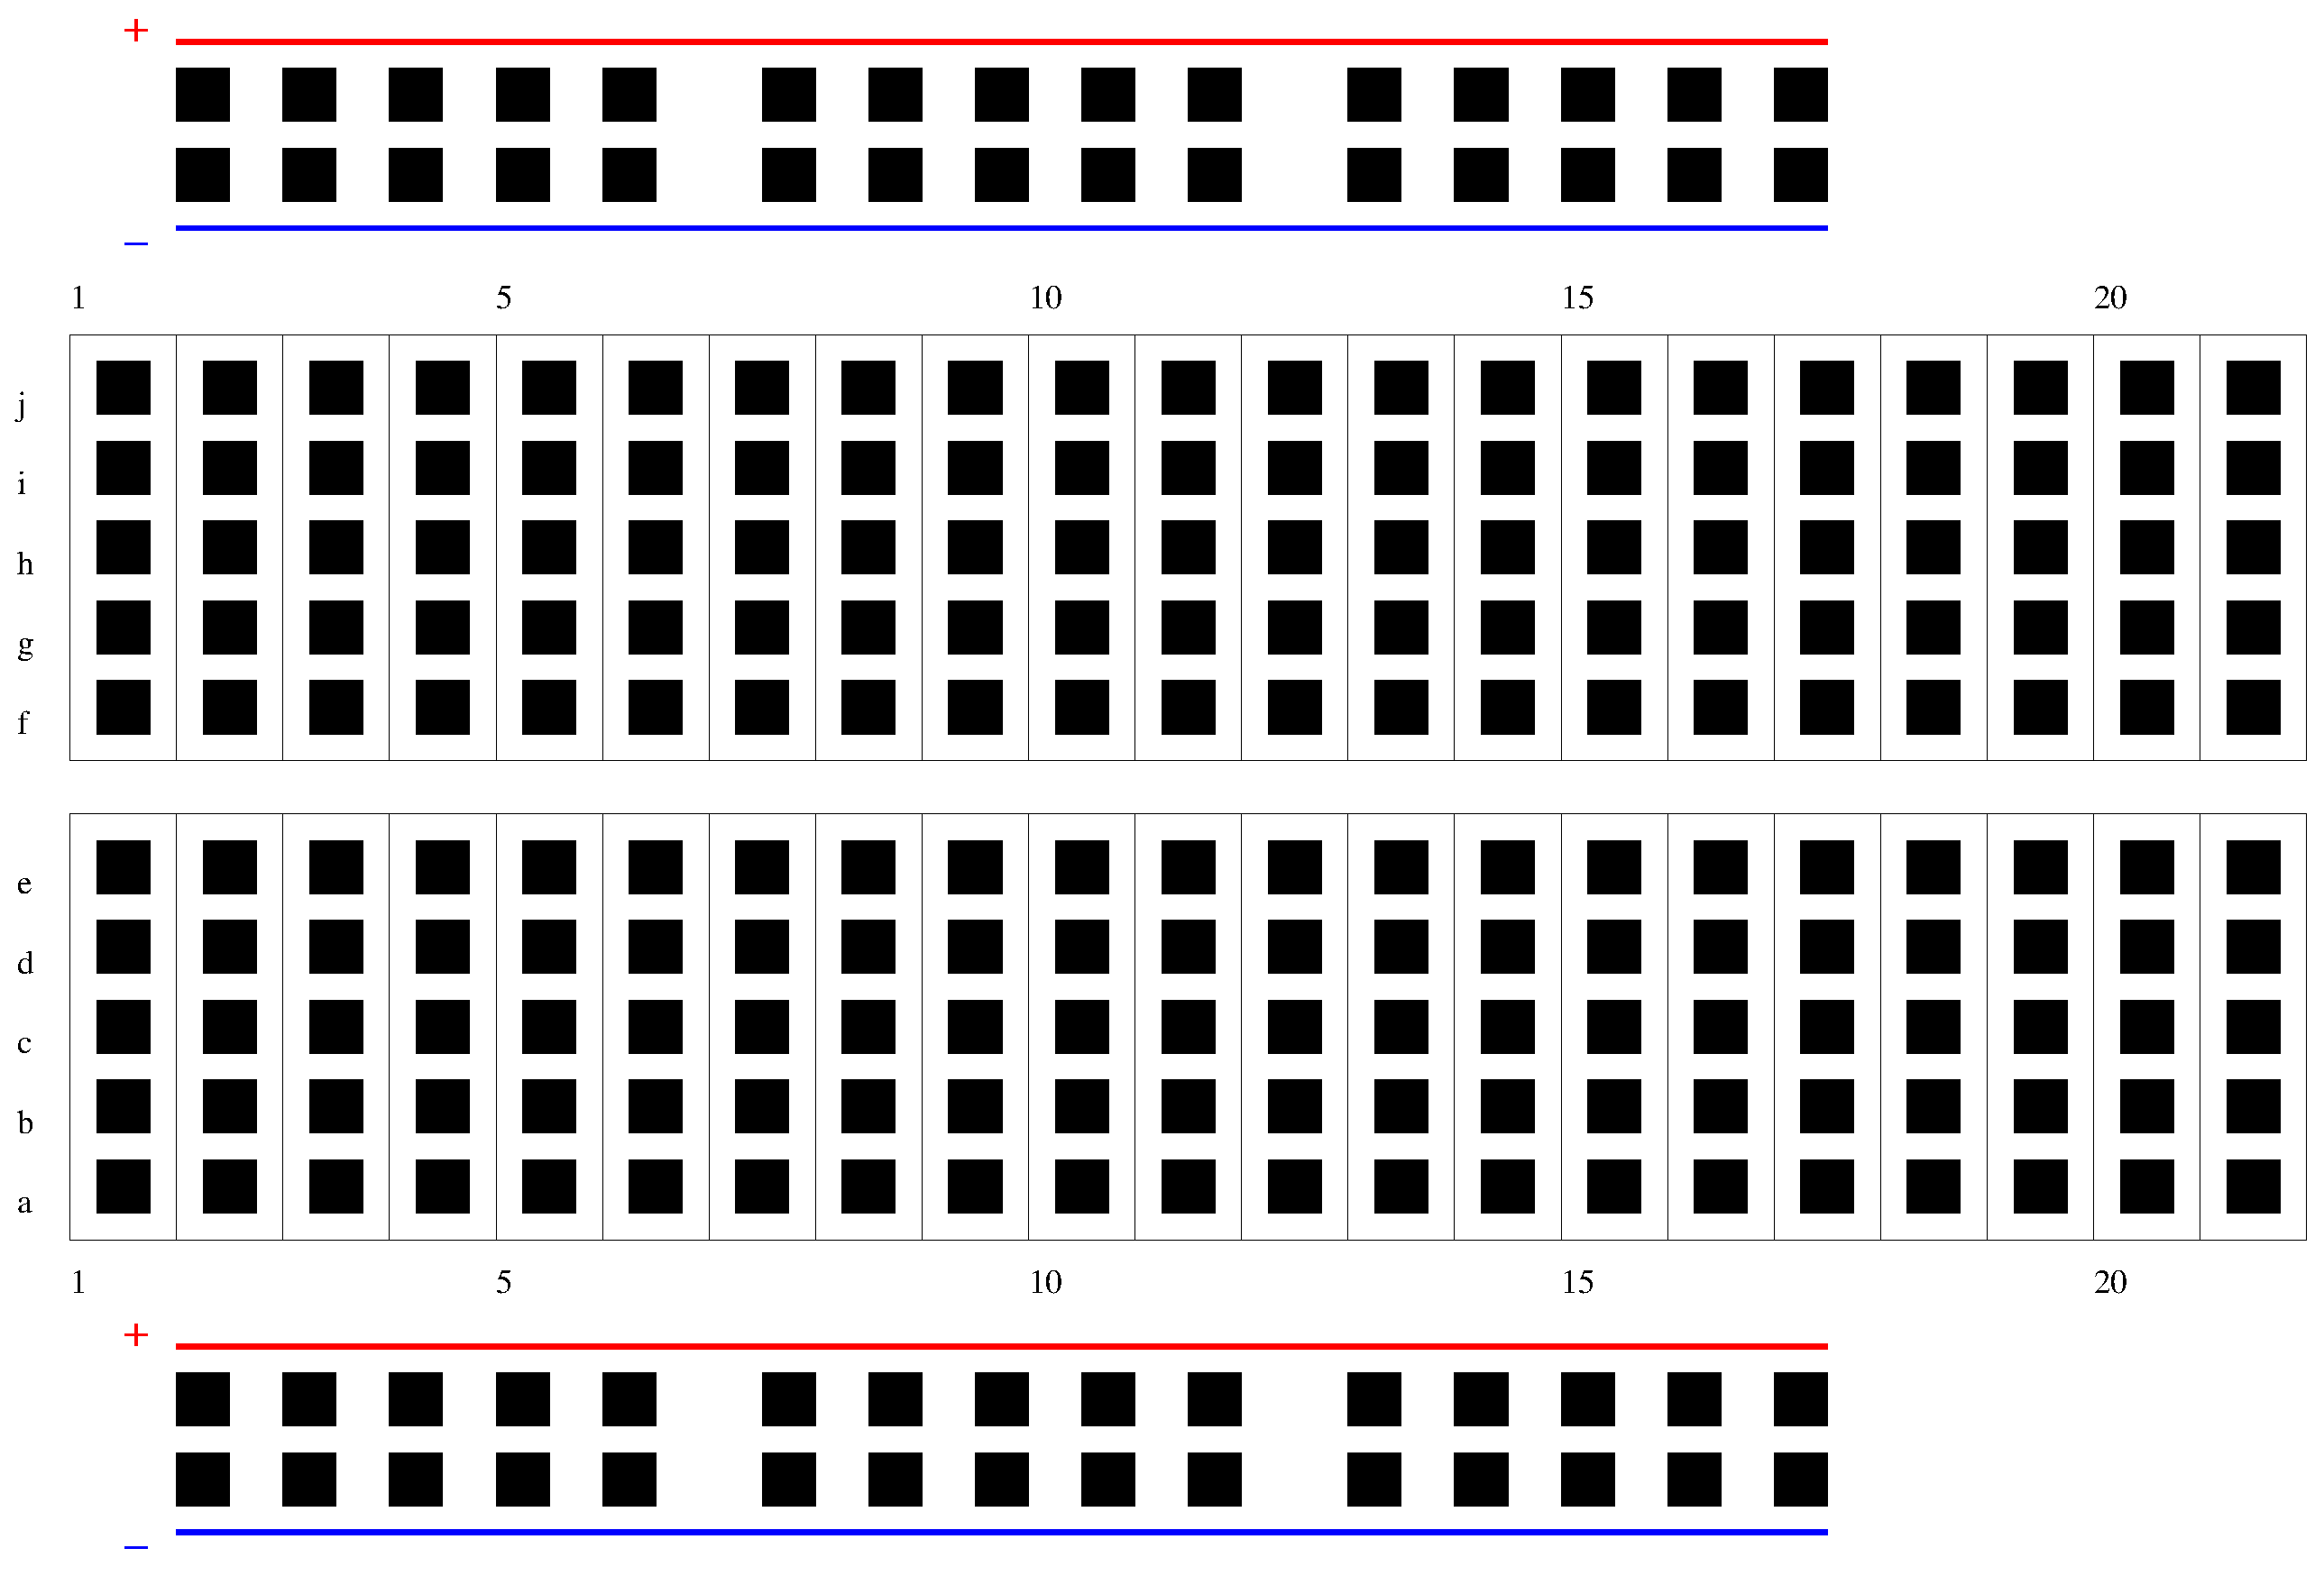
\includegraphics[width=0.7\linewidth]{figures/breadboard.eps}
  \caption{Breadboard
  \label{fig:breadboard}}
\end{figure}

Breadboards will help us to build circuits. It allows for effective connection between components without worrying about the electrical subtleties or hazards. Taking Figure~\ref{fig:breadboard} as a reference, the breadboard has internal electrical connections that makes it possible to tie multiple components to a single point. It does so by representing a \emph{physical} connection as multiple rows of the same column. That is: holes $1$a and $1$d are physically connected inside the breadboard's circuitry, whereas $3$d and $4$a are not.

Each breadboard is divided by thick spaces among different sections. In Figure~\ref{fig:breadboard}, there are four distinct sections: two with the $+$ and $-$ symbols, and two with numbers and letters. The latter was described above, whereas the former works in the opposite way: holes are connected with other holes in the same row. This section is often used to power the circuit, but more on that further in the practice.

Before writing any code, try to assemble the parts as shown in Figure~\ref{fig:blinkingLEDAdvancedLayout}.

\begin{figure}[htbp]
  \centering
  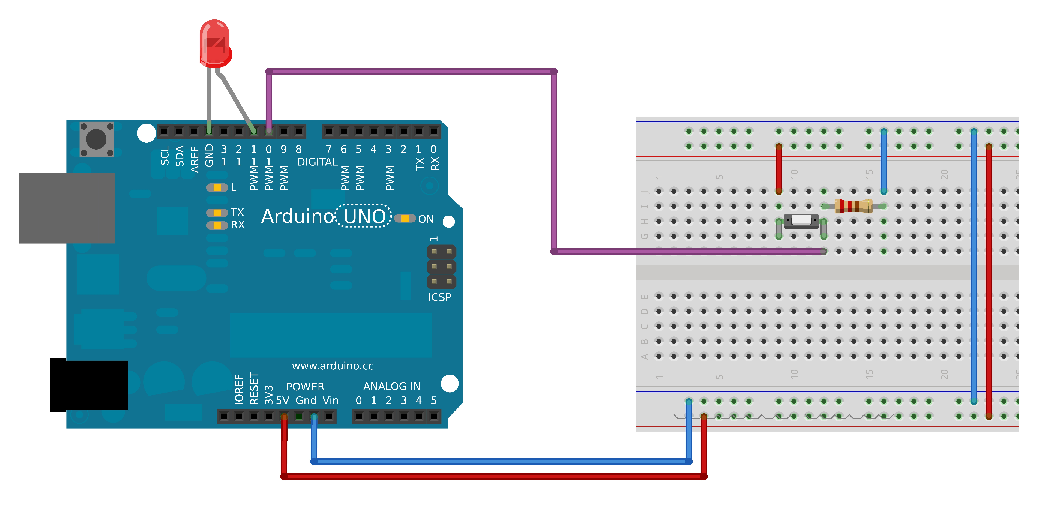
\includegraphics[width=0.9\linewidth]{figures/blinkingLEDAdvanced-NEW.eps}
  \caption{Blinking LED advanced layout
  \label{fig:blinkingLEDAdvancedLayout}}
\end{figure}

To avoid any confusion, let's review the layout component by component:

\begin{enumerate}
	\item Place the pushbutton on your breadboard. In Figure~\ref{fig:blinkingLEDAdvancedLayout}, the two pushbutton "legs" are inserted into holes $5$c and $6$c. In this example, the pushbutton will be energised through the $5$c leg.
	\item Connect one of the legs of the resistor to the negative leg of the pushbutton (hole $6$b). This will physically connect the resistor to one of the legs of the pushbutton. Insert the other leg on hole $9$b.
	\item In order to avoid confusion, cables on all figures are color coded. \emph{Red} represents power cables, \emph{blue} are connections to GND and \emph{cyan} are connections to IO pins on the Arduino. Try to duplicate the layout of Figure~\ref{fig:blinkingLEDAdvancedLayout}.
\end{enumerate}

Note that connecting the $+$ row to the Arduino's $5$V pin will provide $5$V to all the $+$ row. The same is true for GND and the $-$ row. This is very useful to avoid running out of $5$V of GND pins.


\subsection{The code}

Type the following instructions as a new file in the Arduino IDE:

\begin{lstlisting} [caption = {Blinking LED advanced example code}, language = C, label = {code:blinkingLEDAdvanced}, numbers = left, escapeinside={@}{@}]
// Turns on LED when pushbuttom is pressed and
// turns it off when pressed again.

const int LED = 11; @\label{BLA:LED}@
const int BUTTON = 10; @\label{BLA:BUTTON}@
int val = 0;@\label{BLA:val}@
int old_val = 0; @\label{BLA:old_val}@
int state = 0; @\label{BLA:state}@

void setup(){
	pinMode(LED, OUTPUT);@\label{BLA:pinModeLED}@
	pinMode(BUTTON, INPUT);@\label{BLA:pinModeBUTTON}@
}

void loop(){
	val = digitalRead(BUTTON);@\label{BLA:digitalRead}@
	
	//check if the button was pushed
	if((val = = HIGH) && (old_val = = LOW)){@\label{BLA:ifState}@
		state = 1 - state;
		delay(10); @\label{BLA:delay}@
	}@\label{BLA:endIfState}@
	
	old_val = val;@\label{BLA:old_valReasignment}@
	if(state = = 1){
		digitalWrite(LED, HIGH); @\label{BLA:turnOn}@
	}else{
		digitalWrite(LED, LOW);
	}
}
\end{lstlisting}

Let's review the code:

\begin{itemize}
	\item Line~\ref{BLA:LED}: sets the pin for the LED.
	\item Line~\ref{BLA:BUTTON}: assigns the input pin where the pushbutton is connected.
	\item Line~\ref{BLA:val}: \texttt{val} is the variable holding the state of the input pin corresponding to the pushbutton.
	\item Line~\ref{BLA:old_val}: \texttt{old\_val} holds \texttt{val}'s previous value.
	\item Line~\ref{BLA:state}: the variable \texttt{state} determines de condition of the LED. $0$ = off and $1$ = on.
	\item Line~\ref{BLA:pinModeLED}: the function \texttt{pinMode()} sets the roll of each pin. In this case, pin \texttt{LED} is set to \texttt{OUTPUT}.
	\item Line~\ref{BLA:pinModeBUTTON}: sets pin \texttt{BUTTON} to \texttt{INPUT}.
	\item Line~\ref{BLA:digitalRead}: asks whether there is any power at the specified pin. It returns HIGH or LOW if the button is being pushed or not, respectively.
	\item Line~\ref{BLA:ifState}: if the button is being pushed, then \texttt{val} = HIGH and \texttt{old\_val} = LOW. This provokes a change in \texttt{state}.
	\item Line~\ref{BLA:delay}: prevents errors in the change of \texttt{state}. Given that \texttt{loop()} repeats several hundred thousand times per second, making the processor wait a little bit allows for a correct reading of the pushbutton.
	\item Line~\ref{BLA:old_valReasignment}: the value of \texttt{val} is now old. Notice that once the LED is turned on, \texttt{val} = \texttt{old\_val} = LOW. Furthermore, \texttt{val} only changes when the button is pushed.
	\item Line~\ref{BLA:turnOn}: turn LED on.
\end{itemize}



\chapter{An introduction to zigbee and 802.15.4}

\backmatter
%
\bibliographystyle{plain}
\bibliography{my_bib}
\end{document}
